Given the learned parameters and an
observation $\sent$, we want to find the best hidden state sequence
$\hseq^*$; this is called \emph{decoding}. There are several ways to define what we mean by the best
$\hseq^*$; for instance, it could be the best assignment to each hidden
variable $\hs_i$, or the best assignment
to the sequence $\hseq$ as a whole.

The first way, normally called \textbf{Posterior decoding}, consists
in picking the highest state posterior for each position in the sequence:
\begin{equation}
\hseq^* = \argmax_{\hs_1 \ldots \hs_N} b_i(\hs_i)
\end{equation}
where $\gamma_i(\hs_i)$ is the posterior probability $P(\hs_i|\sent)$. 
This method does not guarantee that the sequence $\hseq^*$ is a
valid sequence of the model. For instance there might be a transition
probability between two of the best node posteriors with probability
zero. 

The second approach, called \textbf{Viterbi decoding}, consists in
picking the best global hidden state sequence $\hseq$. 
\begin{equation}
\hseq^* = \argmax_{\hseq} \joint.
\end{equation}

Both approaches rely on dynamic programming, making use of the
independence assumptions of the HMM model. They use an alternative
representation of the HMM called a Trellis (Figure~\ref{fig:trellis}). 
\begin{figure}
\centering
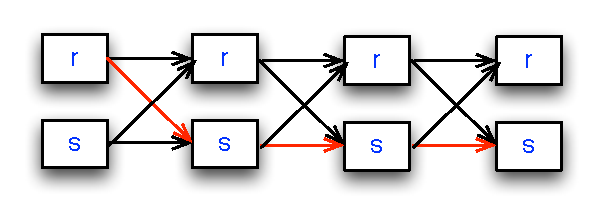
\includegraphics[scale=1]{figs/sequences/trellis}
\caption[HMM Trellis representation.]{\label{fig:trellis} Trellis
  representation of the HMM in Figure ~\ref{hmm}, for the observation
  sequence ``w w s c'', where each hidden variable can take the values $r,s$.}
\end{figure}

This representation unfolds all possible states for each position and
makes explicit the independence assumption: each position only
depends on the previous position. Figure \ref{fig:trellis} shows the
trellis for the particular example in Figure \ref{hmm}. 


Each column represents a position in the sentence, and each row represents a possible state. 
For the decoding algorithms described in the following sections, it is
useful to define a re-parametrization of the model in equation \eqref{eqn:hmm}, in terms of
node potentials $\phi_n(l)$ (associating a number to each box in Figure \ref{fig:trellis})
and edge potentials $\phi_{n-1,n}(l,m)$ (associating a number to each edge in  Figure
\ref{fig:trellis}). For our example, this re-parametrization is given by
%
\begin{equation}
  \joint =\phi_1(r)\phi_1(r,s)\phi_2(s)\phi_2(s,s)\phi_3(s)\phi_3(s,s)\phi_4(s).
  \label{eqn:hmm_ex_treelis}
\end{equation}

%\begin{equation}
%  \joint =\phi_1(``w'',r)\phi_1(r,s)\phi_2(``w'',s)\phi_2(s,s)\phi_3(``s'',s)\phi_3(s,s)\phi_4(``c'',s).
%  \label{eqn:hmm_ex_treelis}
%\end{equation}

In other words, to do this re-parameterization we need to find expressions for the potential variables, (the $\phi$'s) such that \eqref{eqn:hmm} and \eqref{eqn:hmm_ex_treelis} are equal. The solution is given by
\begin{equation}
\phi_{i-1,i}(l,m) = a_{l,m}
\label{eq:nodes1}
\end{equation}
and
\begin{equation}
\phi_i(l) = 
\begin{cases}
 b_{\obs_i}(l)\pi_l \quad\text{i = 1}\\
 b_{\obs_i}(l) \quad\text{i = 2,\ldots,N-1}\\
 b_{\obs_i}(l)a_{l,STOP} \quad\text{i = N}
 \label{eq:nodes2}
\end{cases}
\end{equation}


%\begin{itemize}
%\item\emph{Edge Potentials} - correspond to the transition parameters, with the exception of the
%edges into the last position that correspond to the final transition parameters.
%\item\emph{Node Potentials} - correspond to the observation
%parameters for a given state and the observation at that position.  The
%first position is the exception and corresponds to the
%product between the observation parameters for that state and
%the observation in that position with the initial parameters for that state. 
%\end{itemize}

%Although this re-parametrization simplifies the exposition, and will be
%used in these lectures, it is not necessarily very practical since we
%will be reproducing several values (for instance the transition
%parameters for each position).

\begin{exercise}
Convince yourself that equation \ref{eqn:hmm_ex_treelis} is equivalent to equation \ref{eqn:hmm_ex}, as long as you use the correspondences in equations \eqref{eq:nodes1} and \eqref{eq:nodes2}.

Use the given function \emph{build\_potentials} on the first training sequence and confirm that the values are correct. You should get the same values as presented below.

%Implement a function that builds the node and edge potentials for a
%given sequence. The function head is in the \emph{hmm.py} file:

%\begin{python}
% def build_potentials(self,sequence):
%\end{python}
%
%Run this function for the first training sequence from the simple
%dataset and compare the results given (If the results are the same
%then you are ready to go).

\begin{python}
In[]: run sequences/hmm.py
In[]: hmm = HMM(simple)
In[]: hmm.train_supervised(simple.train)
In[]: node_potentials,edge_potentials = hmm.build_potentials(simple.train.seq_list[0])
In []: node_potentials
Out[]: 
array([[ 0.5       ,  0.75      ,  0.25      ,  0.        ],
       [ 0.08333333,  0.25      ,  0.375     ,  0.140625  ]])
In []: edge_potentials
Out[]: 
array([[[ 0.5  ,  0.5  ,  0.5  ],
        [ 0.5  ,  0.5  ,  0.5  ]],

       [[ 0.   ,  0.   ,  0.   ],
        [ 0.625,  0.625,  0.625]]])
\end{python}
\end{exercise}



\subsection{Posterior Decoding}
Posterior decoding consists
in picking the highest state posterior for each position in the sequence:
\begin{equation}
\hseq^* = \argmax_{\hs_1 \ldots \hs_N} \gamma_i(\hs_i).
\end{equation}

For a given sequence, the \textbf{sequence posterior distribution} is the probability of a particular
hidden state sequence given that we have observed a particular
sentence. Moreover, we will be interested in two other posteriors distributions:
the \textbf{state posterior distribution}, corresponding to the
probability of being in a given state in a certain position given the
observed sentence; the \textbf{transition posterior distribution},
which is the probability of making a particular transition, from position $i$ to
$i+1$ given the observed sentence. 

\begin{align}
  \mathbf{Sequence \ Posterior\!:}\;\;\;\; &\posterior = \frac{\joint}{\marginal}; \label{eq::posteriorDistribution} \\
 \mathbf{State \ Posterior\!:}\;\;\;\;  & \gamma_i(\hv_l) = p_\theta(\hs_i = \hv_l \mid \sent); \label{eq::nodePosterior} \\
 \mathbf{Transition \ Posterior\!:}\;\;\;\;  &\xi_i(\hv_l,\hv_m) = p_\theta(\hs_i = \hv_l, \hs_{i+1}= \hv_m  \mid \sent).\label{eq::edgePosterior}
\end{align}

To compute the posteriors a first step is to be able to compute the 
likelihood of
the sequence $\marginal$, which corresponds to summing the probability of all
possible hidden state sequences.
\begin{equation}
\label{likelihoood}
\mathbf{Likelihood\!:}\;\;\;\; \marginal = \displaystyle \sum_{\hseq} \joint.
\end{equation}
The number of possible hidden state sequences is exponential in the
length of the sentence ($|\hvocab|^N$),
 which makes summing over all of them hard. In this particular small
 example there are $2^4 = 16$ such paths and we can actually enumerate
 them explicitly and calculate their probability using Equation \ref{eqn:hmm_ex_treelis}. But this is as far as it goes, for part-of-speech
 induction with a small tagset of 12 tags and a medium size
 sentence of length 10, there are $12^{10} = 61 917 364 224$ such
 paths. 
Yet, we must be able to compute this sum (sum over $\hseq$) to compute the above likelihood
formula, this is called the inference problem. For sequence models , there is a well know dynamic programming algorithm,
the \textbf{Forward Backward} algorithm (FB), that allows the computation
to be performed in linear time, by making use of the independence assumptions.

The FB algorithm relies on the independence of previous states
assumption, which  
is illustrated in the trellis view by only having arrows between consecutive states. 
The FB algorithm defines two auxiliary probabilities, the forward probability and the backward probability. 
\begin{equation}
\label{eq::forward}
\mathbf{Forward \ Probability\!:}\;\;\;\;  \alpha_i(\hv_l) = p_{\theta}(\hs_i = \hv_l , \obs_1 \ldots \obs_i)
\end{equation}
The forward probability represents the probability that in position
$i$ we are in state $\hs_i = \hv_l$ and that we have observed $\sent$
up to that position. The forward probability is defined by the
following recurrence (we will use the marginals parametrization of the
model): 
\begin{eqnarray}
\alpha_1(\hv_l) &=& \phi_1(l) \\
\alpha_i(\hv_l) &=& \left[ \displaystyle \sum_{\hv_m \in \hvocab} \phi_{(i-1)}(m,l) \alpha_{i-1}(\hv_m) \right] \phi_i(l) \label{forwardRecursion}
\end{eqnarray}

\begin{figure}
\begin{center}
\begin{tabular}{cc}

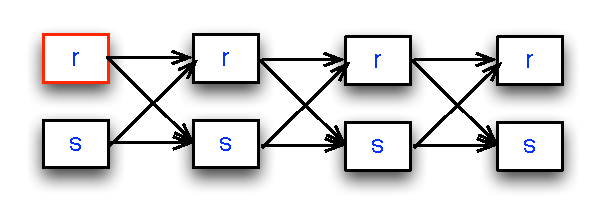
\includegraphics[scale=.5]{figs/sequences/forward1}
& 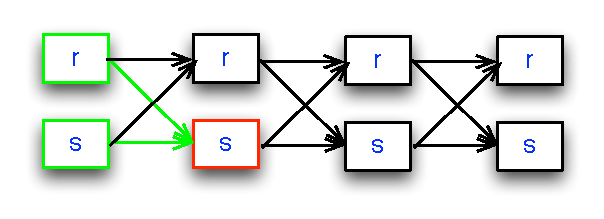
\includegraphics[scale=.5]{figs/sequences/forward2}\\
\end{tabular}
\caption[Forward backward example.]{\label{fig:fb} Forward trellis for
  the first sentence of the training data at position 1 (left) and at
  position 2 (right)}

\end{center}
\end{figure}

At position 1, the probability of being in state ``r'' corresponding
to being in state ``r'' and observing word ``w'' is just the node
marginal for that position $\phi_1(r) = \alpha_1(r)$ (see Figure
 \ref{fig:fb} left). At position 2 the probability
of being in state ``s'' and observing the sequence of words ``w w''
corresponds to the sum of all possible ways of reaching position 2 in
state ``s'' namely: ``rs'' or ``ss'' (see Figure \ref{fig:fb} right). The probability of the first is
$\phi_1(r)\phi_1(r,s)\phi_2(s)$
and the second is $\phi_1(s)\phi_1(s,s)\phi_2(s)$, so:
\begin{eqnarray*}
   \alpha_2(s) &=& \phi_1(r)\phi_1(r,s)\phi_2(s) +
   \phi_1(s)\phi_1(s,s)\phi_2(s) \\
   \alpha_2(s) &=& \left[\phi_1(r)\phi_1(r,s) +
   \phi_1(s)\phi_1(s,s) \right]\phi_2(s) \\
 \alpha_2(s) &=& \displaystyle \sum_{\hs \in \hvocab}
 \left[\phi_1(\hs)\phi_1(\hs,s)\phi_2(s) \right] \\
  \alpha_2(s) &=& \displaystyle \sum_{\hs \in \hvocab}
 \left[\alpha_1(\hs)\phi_1(\hs,s)\phi_2(s) \right]
\end{eqnarray*}

Using the forward trellis one can compute the likelihood by summing
over all possible hidden states for the last position.

\begin{equation}
\label{eq:forwardSum}
\marginal = \displaystyle \sum_{\hseq} \joint = \displaystyle \sum_{\hv \in \hvocab} \alpha_N(\hv) .
\end{equation}

Although the forward probability is enough to calculate the likelihood
of a given sequence, we will also need the backward probability to
calculate the node and edge posteriors. The backward probability,
represents the probability of observing $\sent$ from position $i+1$ up to $N$, given that at position $i$ we are at state $\hs_i = \hv_l$:
 \begin{equation}
\label{eq::backward}
\mathbf{Backward \ Probability\!:}\;\;\;\;  \beta_i(\hv_l) = p_{\theta}(\obs_{i+1}...\obs_N | \hs_i = \hv_l).
\end{equation}
The backward recurrence is given by:
\begin{eqnarray}
\beta_N(\hv_l) &=& 1 \\
\beta_i(\hv_l) &=& \displaystyle \sum_{\hv_m \in \hvocab} \phi_i(l,m)\phi_{i+1}(m) \beta_{i+1}(\hv_m).
%a_{l,m} b_m(\obs_{i+1}) \beta_{i+1}(\hv_m).
\end{eqnarray}
The backward probability is similar to the forward probability, but operates in the inverse direction.
At position $N$ there are no more observations, and the backward
probability is set to 1. At position $i$ the probability 
of having observed the future and being in state $\hv_l$, is given by the sum for all possible states of the probability of having transitioned 
from position $i$ in state $\hv_l$ to position $i+1$ with state $\hv_m$ and observed $\obs_{i+1}$ at time $i+1$ and the future given by  $\beta_{i+1}(\hs_{i+1} = \hv_m)$. 

With the FB probability one can compute the likelihood of a given sentence using any position in the sentence.
\begin{equation}
\label{eq::fbsanity}
  \marginal = \displaystyle \sum_{\hseq} \joint =  \forall{i}
  \displaystyle \sum_{\hv \in \hvocab} \alpha_i(\hv) \beta_i(\hv).
\end{equation}

Note that for time N, $\beta_N(\hv) = 1$ and we get back to equation
\ref{eq:forwardSum}. Although redundant, this fact is useful when implementing an
HMM as a sanity check that the computations are being performed
correctly, since one can compare the likelihood at each position that
should be the same. The FB algorithm may fail for long
sequences since the nested multiplication of numbers smaller than 1
may easily become smaller than the machine precision. To avoid that
problem, \cite{rabiner} presents a scaled version of the FB algorithm that avoids this problem.

Algorithm \ref{alg:fb} shows the pseudo code for the forward backward algorithm.

\begin{algorithm}[t]
   \caption{Forward Backward algorithm \label{alg:fb}}
\begin{algorithmic}[1]
   \STATE {\bfseries input:} sentence $\sent$, parameters $\theta$
        \STATE  \emph{Forward pass}: Compute the forward probabilities
        \STATE \emph{Initialization}
        \FOR{$\hv_l \in \hvocab$ }
        \STATE $\alpha_1(\hv_l) = \phi_1(\hv_l)$
        \ENDFOR 
        \FOR{$i=2$ {\bfseries to} $N$}
         \FOR{$\hv_l \in \hvocab$ }
                 \STATE $\alpha_i(\hv_l) = \left[ \displaystyle
                   \sum_{m  \in \hvocab} \phi_{(i-1)}(m,l)
                   \alpha_{i-1}(\hv_m) \right] \phi_i(l)$
         \ENDFOR 
        \ENDFOR 
       \STATE \emph{Backward pass}: Compute the backward probabilities
       \STATE \emph{Initialization}
        \FOR{$\hv_l \in \hvocab$ }
        \STATE $\beta_N(\hv_l) = 1$
        \ENDFOR 
       \FOR{$i=N-1$ {\bfseries to} 1}
        \STATE $\beta_i(\hv_l) = \displaystyle \sum_{\hv_m \in \hvocab} \phi_i(l,m)\phi_{i+1}(m) \beta_{i+1}(\hv_m).$
        \ENDFOR 
       \STATE \textbf{output:} The forward and backward probabilities
       $\alpha$ and $\beta$
\end{algorithmic}
\end{algorithm}



\begin{exercise}
Given the implementation of the forward pass of the forward backward
algorithm in the file \emph{forward\_backward.py} implement the backward pass.
\begin{python}

def forward_backward(node_potentials,edge_potentials):
    H,N = node_potentials.shape
    forward = np.zeros([H,N],dtype=float)
    backward = np.zeros([H,N],dtype=float)
    forward[:,0] = node_potentials[:,0]
    ## Forward loop
    for pos in xrange(1,N):
        for current_state in xrange(H):
            for prev_state in xrange(H):
                forward_v = forward[prev_state,pos-1]
                trans_v = edge_potentials[prev_state,current_state,pos-1]
                prob = forward_v*trans_v
                forward[current_state,pos] += prob
            forward[current_state,pos] *= node_potentials[current_state,pos]
    ## Backward loop
          ## Your code
   return forward,backward

\end{python}

Use the provided function that makes use of Equation \ref{eq::fbsanity} to make
sure your implementation is correct:
 
\begin{python}
In[]:  run sequences/hmm.py
In[]: hmm = HMM(simple)
In[]: hmm.train_supervised(simple.train)
In[]: forward,backward =  hmm.forward_backward(simple.train.seq_list[0])
In []: sanity_check_forward_backward(forward,backward)
Out[]: 
array([[ 0.03613281],
       [ 0.03613281],
       [ 0.03613281],
       [ 0.03613281]])
\end{python}
\end{exercise}

Moreover, given the forward and backward probabilities one can compute both the state
and transition posteriors.

\begin{align}
 \mathbf{State \ Posterior\!:}\;\;\;\;   \gamma_i(\hv_l) &= p_\theta(\hs_i = \hv_l \mid \sent) = \frac{\alpha_i(\hv_l) \beta_i(\hv_l)}{\marginal}; \label{eq::nodePosterior2} \\
 \mathbf{Transition \ Posterior\!:}\;\;\;\;  \xi_i(\hv_l,\hv_m) &= p_\theta(\hs_i = \hv_l, \hs_{i+1}= \hv_m  \mid \sent) \nonumber\\
 &=  \frac{\alpha_i(\hv_l) \phi_i(l,m)\phi_{i+1}(m)\beta_{i+1}(\hv_m)}{\marginal}.\label{eq::edgePosterior2}
\end{align}
A graphical representation of these posteriors is illustrated in figure~\ref{fig:posteriors}. 
On the left it is shown that $\alpha_i(\hv_l) \beta_i(\hv_l)$ returns the sum of all paths that contain the state $y_i$, weighted by $\joint$, and on the right we can see that $\alpha_i(\hv_l) \phi_i(l,m)\phi_{i+1}(m)\beta_{i+1}(\hv_m)$ returns the same for all paths containing the edge from $y_l$ to $y_m$.
Thus, these posteriors can be seen as the ratio of the number of paths that contain the given state or transition (weighted by $\joint$) and the number of possible paths in the graph $\marginal$.
As an practical example, given that the person perform the sequence of actions ``w w s c", we want to know the probability of having been raining in the second day. The state posterior probability for this event can be seen as the probability that the sequence of actions ``walk walk shop clean" was generated by a sequence of weathers and where it was raining in the second day. In this case, the possible sequences would be "r r r r", "s r r r", "r r s r", "r r r s", "s r s r", "s r r s", "r r s s", and "s r s s".

\begin{figure}
\begin{center}
\begin{tabular}{cc}

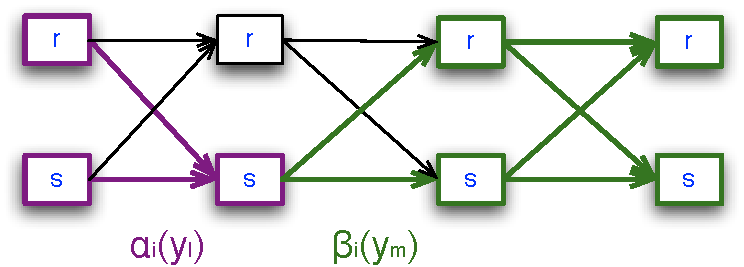
\includegraphics[scale=.5]{figs/sequences/statePost}
& 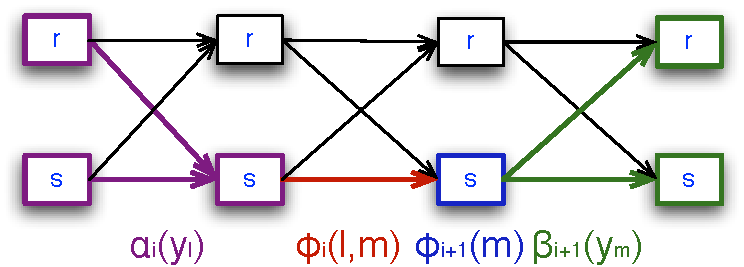
\includegraphics[scale=.5]{figs/sequences/transPost}\\
\end{tabular}
\caption[Posterior Illustration.]{\label{fig:posteriors} A graphical representation of the components in the state and transition posteriors.}

\end{center}
\end{figure}

Using the node posteriors we are ready to perform posterior
decoding. Algorithm \ref{alg:pd} shown the posterior decoding algorithm.

\begin{algorithm}[t]
   \caption{Posterior Decoding algorithm \label{alg:pd}}
\begin{algorithmic}[1]
   \STATE {\bfseries input:} The forward and backward probabilities
       $\alpha$ and $\beta$.
   \STATE  \emph{Compute Likelihood}: Compute the likelihood of the
   sentence
   \STATE $L = 0$
   \FOR{$\hv_l \in \hvocab$ }
   \STATE $\marginal = \marginal + \alpha_N(\hv_l)$
   \ENDFOR 
   \STATE $\hat \hseq = []$
    \FOR{$i=1$ {\bfseries to} $N$}
    \STATE $max = 0$
     \FOR{$\hv_l \in \hvocab$ }
     \STATE $\gamma_i(\hv_l)  =  \frac{\alpha_i(\hv_l)
       \beta_i(\hv_l)}{\marginal}$
     \IF {$\gamma_i(\hv_l) > max$}
     \STATE $max = \gamma_i(\hv_l)$
     \STATE $\hat  y_i = \hv_l$
     \ENDIF
     \ENDFOR 
     \ENDFOR 
   \STATE \textbf{output:} the posterior path $\hat \hseq$
\end{algorithmic}
\end{algorithm}



\begin{exercise}
Given the node and edge posterior formulas \ref{eq::nodePosterior},\ref{eq::edgePosterior} and the
  forward and backward formulas \ref{eq::forward},\ref{eq::backward} convince yourself that formulas
  \ref{eq::nodePosterior2},\ref{eq::edgePosterior2} are correct. 

Compute the node posteriors for the first training sentence, and look at
the output. Can you come up with a sanity check for calculating the
posteriors (Hint: Note that the node posteriors are a proper
probability distribution).

\begin{python}
In[]:  run sequences/hmm.py
In[]: hmm = HMM(simple)
In[]: hmm.train_supervised(simple.train)
In [15]: node_posteriors = hmm.get_node_posteriors(simple.train.seq_list[0])

In [16]: node_posteriors
Out[16]: 
array([[ 0.91891892,  0.75675676,  0.43243243,  0.        ],
       [ 0.08108108,  0.24324324,  0.56756757,  1.        ]])
\end{python}

Implement the posterior decode method using the method you tried previously. 
\begin{python}
def posterior_decode(self,seq):
\end{python}

Run the posterior decode on the first test sequence, and evaluate it.
 
\begin{python}
In[]:  run sequences/hmm.py
In[]: hmm = HMM(simple)
In[]: hmm.train_supervised(simple.train)
In [19]: y_pred = hmm.posterior_decode(simple.test.seq_list[0])
In [20]: w/r w/r s/s c/s
Out[20]: array([0, 0, 1, 1])
In [21]: simple.test.seq_list[0]
Out[21]: w/r w/s s/s c/s
\end{python}

Do the same for the second test sentence:
\begin{python}
In [22]: y_pred = hmm.posterior_decode(simple.test.seq_list[1])
In [23]: y_pred
Out[23]: c/r w/r t/r w/r
In [24]: simple.test.seq_list[1]
Out[24]: c/s w/s t/s w/s 
\end{python}

What is wrong? Observe the observations for that sentence. In fact the
observation t was never seen at training time, so the probability for
it will be zero (no matter what state) and make all possible state
sequences have zero probability (the value 0 is just the default.
As seen in the previous lecture, this is a problem with generative
models, that can be corrected using smoothing (there are other
options).

Change your train method to add smoothing:
\begin{python}
def train_supervised(self,sequence_list, smoothing):
\end{python}

Repeat the last exercise with the new parameters. What do you observe?
\end{exercise}


Note that if you use smoothing when training you need to account for
that in the counts sanity checks you did in the previous exercise.

\begin{exercise}
Change the function you just created \emph{ def
  sanity\_check\_counts(self,seq\_list):} to account for smoothing. Make
sure it works properly.

\begin{python}
In []: run sequences/hmm.py
In []: hmm = HMM(simple)
In []: hmm.collect_counts_from_corpus(simple.train,smoothing=0.1)
In []: hmm.sanity_check_counts(simple.train,smoothing=0.1)
Init Counts match
Final Counts match
Transition Counts match
Observations Counts match
\end{python}
\end{exercise}


\subsection{Viterbi Decoding}


\textbf{Viterbi decoding} consists in
picking the best global hidden state sequence $\hseq$. 
\begin{equation}
\hseq^* = \argmax_{\hseq} \joint.
\end{equation}

The viterbi algorithm 
is very similar to the forward procedure of the FB algorithm,
making use of the same trellis structure to efficiently represent and 
use all the exponential number of sequences. In fact the only
difference from the forward algorithm is in the recursion
\ref{forwardRecursion} where instead of summing over all possible 
hidden states, we take their maximum.

\begin{equation}
\label{eq::viterbi}
\mathbf{Viterbi }\;\;\;\;  \delta_i(\hv_l) = \argmax_{y_1...y_i} p_{\theta}(\hs_i = \hv_l , \obs_1 \ldots \obs_i)
\end{equation}
The viterbi trellis represents the path with maximum probability in
position
$i$ when we are in state $\hs_i = \hv_l$ and that we have observed $\sent$
up to that position. The viterbi algorithm is defined by the
following recurrence (we will use the marginals parametrization of the
model): 
\begin{eqnarray}
\delta_1(\hv_l) &=& \phi_1(l) \\
\delta_i(\hv_l) &=& \left[ \max_{y_1 ... y_i} \phi_{(i-1)}(m,l)
  \delta_{i-1}(\hv_m) \right] \phi_i(l) \label{viterbiRecursion} \\
\psi_{i}(\hv_l) &=& \left[ \argmax_{y_1 ... y_i} \right]
%\phi_{(i-1)}(m,l)  \delta_{i-1}(\hv_m) \right] \phi_i(l) \label{viterbiBackpointers}
\end{eqnarray}

Algorithm \ref{alg:viterbi} shows the pseudo code for the Viterbi algorithm.
\begin{algorithm}[t]
   \caption{Viterbi algorithm \label{alg:viterbi}}
\begin{algorithmic}[1]
   \STATE {\bfseries input:} sentence $\sent$, parameters $\theta$
        \STATE  \emph{Forward pass}: compute the maximum paths for
        every end state
        \STATE \emph{Initialization}
        \FOR{$\hv_l \in \hvocab$ }
        \STATE $\delta_1(\hv_l) = \phi_1(\hv_l)$
        \ENDFOR 
        \FOR{$i=2$ {\bfseries to} $N$}
         \FOR{$\hv_l \in \hvocab$ }
                 \STATE $\delta_i(\hv_l) = \left[ \displaystyle
                   \max_{m  \in \hvocab} \phi_{(i-1)}(m,l)
                   \delta_{i-1}(\hv_m) \right] \phi_i(l)$
                 \STATE $\psi_{i}(\hv_l) = m$
         \ENDFOR 
        \ENDFOR 
       \STATE \emph{Backward pass}: Build the most likely path
       \STATE $\hat \hseq = []$ 
       \STATE $\hat y_N = \displaystyle \argmax_{\hv_m  \in
                   |\hvocab |}  \delta_N(\hv_l)$
       \FOR{$i=N$ {\bfseries to} 2}
        \STATE $\hat  y_i = \psi_{i+1}(y_{i+1})$
        \ENDFOR 
       \STATE \textbf{output:} the viterbi path $\hat \hseq$
\end{algorithmic}
\end{algorithm}


\begin{exercise}
Implement a method for performing viterbi decoding.
\begin{python}
        def viterbi_decode(self,seq):
\end{python}

Test your method on both test sentences and compare the results with
the ones given.
\begin{python}
In []: y_pred = hmm.viterbi_decode(simple.test.seq_list[0])
In []: y_pred
Out[]: w/r w/r s/r c/s 
In []: y_pred = hmm.viterbi_decode(simple.test.seq_list[1])
In []: y_pred
Out[]: c/r w/r t/r w/r 
\end{python}
\end{exercise}




%%% Local Variables: 
%%% mode: latex
%%% TeX-master: "../../guide"
%%% End: 
